% !TEX root = ../main.tex

\chapter{Appendix}

\section*{HPLC Methods} % (fold)
\label{sec:hplc_methods}

	Vielleicht wenn hier text steht

	\begin{table}[htbp]
		\caption[Standard aminocolumn method]{\textbf{Standard Screening Method}}
		\label{tab:method_c18_screening}
		\centering
		\begin{tabularx}{\textwidth}{XX}
			\toprule
			\textbf{Parameter}	& \textbf{Value}	\\
			\midrule
			Column 		& Nucleosil-100 C18 \SI{5}{\micro\meter} 150$\times$\SI{3}{\milli\meter} 	\\
			Solvents	& A: Water + 0.1~\% Formic acid 	\\
						& B: Acetonitrile + 0.1~\% Formic acid		\\
			Method 		& Gradient 5 - 100 \% B for \SI{15}{\minute} 	\\
						& Plateau 100 \% B for \SI{3}{\minute} 	\\
			Flow 		& \SI{1.25}{\milli\liter\per\minute} \\
			Temperature & \SI{25}{\celsius} 	\\
			Injection Volume 	& \SI{50}{\micro\liter} 	\\
			\bottomrule
		\end{tabularx}
	\end{table}

	\begin{table}[htbp]
		\caption[Standard aminocolumn method]{\textbf{Standard aminocolumn method}}
		\label{tab:method_nh2_standard}
		\centering
		\begin{tabularx}{\textwidth}{XX}
			\toprule
			\textbf{Parameter}	& \textbf{Value}	\\
			\midrule
			Column 		& Luna NH2 \SI{5}{\micro\meter} 250$\times$\SI{4.6}{\milli\meter} 	\\
			Solvents	& A: Water + 0.1~\% Formic acid 	\\
						& B: Acetonitrile + 0.1~\% Formic acid		\\
			Method 		& Isocratic 80~\% B for \SI{20}{\minute} 	\\
						& + 100~\% A for \SI{10}{\minute}   \\
			Flow 		& \SI{2}{\milli\liter\per\minute} \\
			Temperature & \SI{25}{\celsius} 	\\
			Injection Volume 	& \SI{50}{\micro\liter} 	\\
			\bottomrule
		\end{tabularx}
	\end{table}

	\begin{table}[htbp]
		\caption[The standard HILIC method]{\textbf{The standard HILIC method}}
		\label{tab:method_hilic_standard}
		\centering
		\begin{tabularx}{\textwidth}{XX}
			\toprule
			\textbf{Component}	& \textbf{Parameter}	\\
			\midrule
			Column 		& ZIC-HILIC \SI{3.5}{\micro\meter} 150$\times$\SI{4.6}{\milli\meter} 	\\
			Solvents	& A: 	10~mM Ammonium acetate 	\\
						& B: 	Acetonitrile 			\\
			Method 		& Isocratic 80~\% B for 45 min. 	\\
			Flow 		& \SI{0.8}{\milli\liter\per\minute} \\
			Temperature & \SI{25}{\celsius} 	\\
			Injection Volume 	& \SI{50}{\micro\liter} 	\\
			\bottomrule
		\end{tabularx}
	\end{table}

	\begin{table}[htbp]
		\caption[Standard aminocolumn method]{\textbf{HILIC method adapted for MS coupling}}
		\label{tab:method_hilic_ms}
		\centering
		\begin{tabularx}{\textwidth}{XX}
			\toprule
			\textbf{Component}	& \textbf{Parameter}	\\
			\midrule
			Column 		& ZIC-HILIC \SI{3.5}{\micro\meter} 150$\times$\SI{4.6}{\milli\meter} 	\\
			Solvents	& A: 	10~mM Ammonium acetate 	\\
						& B: 	Acetonitrile 			\\
			Method 		& Isocratic 80~\% B for 60 min. 	\\
			Flow 		& \SI{0.5}{\milli\liter\per\minute} \\
			Temperature & \SI{40}{\celsius} 	\\
			Injection Volume 	& \SI{50}{\micro\liter} 	\\
			\bottomrule
		\end{tabularx}
	\end{table}

	\begin{table}[htbp]
		\caption[Screening method for HPLC-MS]{\textbf{Screening method for HPLC-MS}}
		\label{tab:method_ms_1}
		\centering
		\begin{tabularx}{\textwidth}{XX}
			\toprule
			\textbf{Parameter}	& \textbf{Value}	\\
			\midrule
			Column 		& Nucleosil-100 \SI{5}{\micro\meter} 150$\times$\SI{3}{\milli\meter} 	\\
			Solvents	& A: Water + 0.1~\% Formic acid 	\\
						& B: Acetonitrile + 0.06~\% Formic acid		\\
			Method 		& Gradient 0 - 100 \% B for \SI{15}{\minute} 	\\
						& Plateau 100 \% B for \SI{2}{\minute} 	\\
			Flow 		& \SI{0.4}{\milli\liter\per\minute} \\
			Temperature & \SI{40}{\celsius} 	\\
			Injection Volume 	& \SI{2.5}{\micro\liter} 	\\
			\midrule
			Capillary Voltage 	& \SI{3500}{\volt} 	\\
			Injector Temperature& \SI{350}{\celsius}\\
			Target mass 		& 400 m/z 			\\
			\bottomrule
		\end{tabularx}
	\end{table}

	\begin{table}[htbp]
		\caption[Screening Method Polar-C18]{\textbf{Screening Method Polar-C18}}
		\label{tab:method_polarc18_screening}
		\centering
		\begin{tabularx}{\textwidth}{XX}
			\toprule
			\textbf{Parameter}	& \textbf{Value}	\\
			\midrule
			Column 		& Kinetex Polar-C18 \SI{2.6}{\micro\meter} 150$\times$\SI{4.6}{\milli\meter} 	\\
			Solvents	& A: Water + 0.1~\% Formic acid 	\\
						& B: Acetonitrile + 0.1~\% Formic acid		\\
			Method 		& Gradient 5 - 100 \% B for \SI{20}{\minute} 	\\
						& Plateau 100 \% B for \SI{6}{\minute} 	\\
			Flow 		& \SI{1.2}{\milli\liter\per\minute} \\
			Temperature & \SI{50}{\celsius} 	\\
			Injection Volume 	& \SI{50}{\micro\liter} 	\\
			\bottomrule
		\end{tabularx}
	\end{table}

	\begin{table}[htbp]
		\caption[Reverse Screening Method Polar-C18]{\textbf{Reverse Screening Method Polar-C18}}
		\label{tab:method_polarc18_revscreening}
		\centering
		\begin{tabularx}{\textwidth}{XX}
			\toprule
			\textbf{Parameter}	& \textbf{Value}	\\
			\midrule
			Column 		& Kinetex Polar-C18 \SI{2.6}{\micro\meter} 150$\times$\SI{4.6}{\milli\meter} 	\\
			Solvents	& A: Water + 0.1~\% Formic acid 	\\
						& B: Acetonitrile + 0.1~\% Formic acid		\\
			Method 		& Gradient 100 - 5 \% B for \SI{20}{\minute} 	\\
						& Plateau 100 \% B for \SI{6}{\minute} 	\\
			Flow 		& \SI{1.2}{\milli\liter\per\minute} \\
			Temperature & \SI{50}{\celsius} 	\\
			Injection Volume 	& \SI{50}{\micro\liter} 	\\
			\bottomrule
		\end{tabularx}
	\end{table}

% section hplc_methods (end)

\section*{Genomic analysis} % (fold)
\label{sec:genomic_analysis}

    \begin{figure}[htpb]
        \centering
        \begin{subfigure}[b]{\textwidth}
            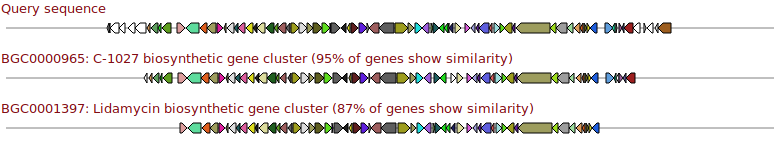
\includegraphics[width=1\linewidth]{contig4_cluster_search}
            \caption{Cluster search results for the identified cluster.}
            \label{fig:sub1}
        \end{subfigure}

        \begin{subfigure}[b]{\textwidth}
            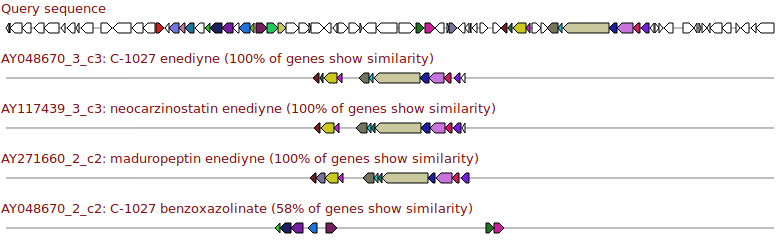
\includegraphics[width=1\linewidth]{contig4_subcluster_search}
            \caption{Subcluster search results for the identified cluster.}
            \label{fig:sub2}
        \end{subfigure}

        \caption[Cluster and subcluster search results for the cluster located on contig four.]{\textbf{Cluster and subcluster search results for the cluster located on contig four.} The 160~kb contig was submitted to AntiSMASH with the ClusterFinder option. Only the search results with the highest similarities are shown.}
        \label{fig:cluster_search}
    \end{figure}

% section genomic_analysis (end)
